% jquantstats.tex — companion paper for the jQuantStats library
\documentclass[11pt,a4paper]{article}

% --------------------------------------------------------------------------
% Packages
% --------------------------------------------------------------------------
\usepackage[T1]{fontenc}
\usepackage[utf8]{inputenc}
\usepackage{lmodern}
\usepackage{microtype}
\usepackage[a4paper, margin=2.5cm]{geometry}

% Mathematics
\usepackage{amsmath}
\usepackage{amssymb}
\usepackage{amsthm}
\usepackage{bm}

% Tables
\usepackage{booktabs}
\usepackage{array}
\usepackage{longtable}

% Graphics
\usepackage{graphicx}
\usepackage{xcolor}
\usepackage{tikz}

% Code listings
\usepackage{listings}
\usepackage{caption}
\usepackage{subcaption}

% Lists
\usepackage{enumitem}

% References
\usepackage[round]{natbib}
\usepackage[colorlinks=true, linkcolor=blue!60!black, citecolor=blue!60!black,
            urlcolor=blue!60!black]{hyperref}

% --------------------------------------------------------------------------
% Custom macros
% --------------------------------------------------------------------------
\newcommand{\R}{\mathbb{R}}
\newcommand{\E}{\mathbb{E}}
\newcommand{\Var}{\operatorname{Var}}
\newcommand{\Cov}{\operatorname{Cov}}
\newcommand{\sr}{\widehat{\mathrm{SR}}}
\newcommand{\rvec}[1]{\bm{#1}}
\DeclareMathOperator{\sgn}{sgn}

% Theorem environments
\newtheorem{remark}{Remark}
\newtheorem{proposition}{Proposition}
\newtheorem{definition}{Definition}

% --------------------------------------------------------------------------
% Code listing style
% --------------------------------------------------------------------------
\definecolor{codegray}{rgb}{0.95,0.95,0.95}
\definecolor{codegreen}{rgb}{0.0,0.45,0.0}
\definecolor{codepurple}{rgb}{0.45,0.0,0.6}
\definecolor{codeblue}{rgb}{0.0,0.0,0.7}

\lstset{
  language=Python,
  backgroundcolor=\color{codegray},
  basicstyle=\ttfamily\small,
  keywordstyle=\color{codeblue}\bfseries,
  stringstyle=\color{codepurple},
  commentstyle=\color{codegreen}\itshape,
  numbers=left,
  numberstyle=\tiny\color{gray},
  numbersep=8pt,
  frame=single,
  framerule=0.4pt,
  breaklines=true,
  captionpos=b,
  tabsize=4,
  showstringspaces=false,
}

% --------------------------------------------------------------------------
% Document
% --------------------------------------------------------------------------
\begin{document}

\title{%
  \textbf{jQuantStats: Portfolio Analytics for Quants}\\[0.4em]
  {\large A Companion Paper}
}
\author{Jebel Quant}
\date{March 2026}

\maketitle

\begin{abstract}
\noindent
\textbf{jQuantStats} is an open-source Python library for portfolio performance
analytics designed for systematic traders and quantitative portfolio managers.
It provides a comprehensive suite of over eighty risk and return metrics,
interactive Plotly visualisations, and an HTML reporting engine, all built on a
modern, Polars-native stack with zero pandas runtime dependency.

The library exposes two entry points: \texttt{Portfolio}, which ingests raw
price series and position sizes to compute transaction-cost-aware performance
metrics, and \texttt{Data}, which operates on pre-computed return streams.
Both surfaces share a unified \texttt{Stats} facade that covers descriptive
statistics, drawdown analysis, risk-adjusted ratios, benchmark attribution, and
rolling analytics.

This paper documents the design rationale, mathematical foundations, and
practical usage of the library.  It serves as a reference for practitioners who
wish to understand the precise definitions underlying each metric, the
Brinson-style tilt/timing attribution model, the two-factor transaction cost
framework, and the conventions used to annualise statistics across different
return frequencies.
\end{abstract}

\tableofcontents
\newpage

% ==========================================================================
\section{Introduction}
\label{sec:intro}
% ==========================================================================

Quantitative practitioners routinely need to evaluate a strategy's historical
performance across many dimensions: raw return, risk-adjusted return, drawdown
characteristics, benchmark sensitivity, concentration, and trading costs.
Existing open-source tools such as \texttt{QuantStats} \citep{quantstats2019}
were built on pandas and matplotlib and reflect the conventions of an earlier
era of Python data science.

\textbf{jQuantStats} was written from scratch to address three structural
limitations of that generation of tools.

\begin{enumerate}[leftmargin=*, label=\arabic{*}.]
  \item \textbf{DataFrame backend.}  Pandas carries significant overhead for
    columnar workloads that arise in portfolio analytics.  jQuantStats uses
    Polars \citep{polars2024} as its primary engine, reducing memory usage and
    improving throughput on large price histories.  The public API is mediated
    through Narwhals \citep{narwhals2024}, a lightweight abstraction layer that
    accepts both Polars and pandas frames at system boundaries.
  \item \textbf{Visualisation.}  Static matplotlib figures are unsuitable for
    interactive analysis.  Every chart in jQuantStats is rendered with Plotly,
    producing fully interactive HTML widgets that can be embedded in notebooks,
    dashboards, or self-contained HTML reports.
  \item \textbf{Type safety.}  The library targets Python~3.11+, is fully
    annotated, ships a \texttt{py.typed} marker, and achieves 100\% docstring
    coverage.  This makes IDE integration and downstream static analysis
    straightforward.
\end{enumerate}

The remainder of this paper is structured as follows.
Section~\ref{sec:arch} describes the two-class architecture and data model.
Section~\ref{sec:stats} derives the mathematical definitions of every metric.
Section~\ref{sec:attribution} presents the Brinson tilt/timing attribution
framework.
Section~\ref{sec:costs} documents the transaction cost models.
Section~\ref{sec:plots} surveys the visualisation and reporting surfaces.
Section~\ref{sec:usage} gives an end-to-end worked example.
Section~\ref{sec:annualisation} discusses frequency detection and annualisation
conventions.
Appendix~\ref{app:api} provides a compact API reference.

% ==========================================================================
\section{Architecture and Data Model}
\label{sec:arch}
% ==========================================================================

\subsection{Entry Points}

The public API consists of two classes.

\paragraph{Portfolio.}
\texttt{Portfolio} is the primary entry point for systematic strategies where
the analyst controls both the signal and the position sizing.  It is constructed
via

\begin{lstlisting}[caption={Constructing a Portfolio from prices and positions.}]
from jquantstats import Portfolio

pf = Portfolio.from_cash_position(
    prices=prices_df,       # Polars DataFrame, one column per instrument
    cash_position=pos_df,   # signed cash notional per instrument per day
    aum=1_000_000,          # total assets under management
    cost_per_unit=0.0,      # optional: GBP per share traded
    cost_bps=0.0,           # optional: basis points of AUM turnover
)
\end{lstlisting}

\texttt{Portfolio} derives all downstream quantities—daily profit and loss,
net asset value, returns, drawdown series, tilt/timing decomposition, and
turnover—directly from the raw inputs without requiring the caller to pre-process
data.

\paragraph{Data.}
\texttt{Data} is a lighter entry point for analysts working with pre-computed
return streams, for example when evaluating a signal provided by a third party.

\begin{lstlisting}[caption={Constructing a Data object from returns.}]
from jquantstats import Data

d = Data.from_returns(
    returns=returns_series,     # Polars Series of period returns
    rf=0.0,                     # risk-free rate (same frequency as returns)
    benchmark=bench_series,     # optional benchmark returns
)
\end{lstlisting}

\subsection{Internal Data Flow}

Figure~\ref{fig:dataflow} illustrates how raw inputs flow through the library.

\begin{figure}[ht]
\centering
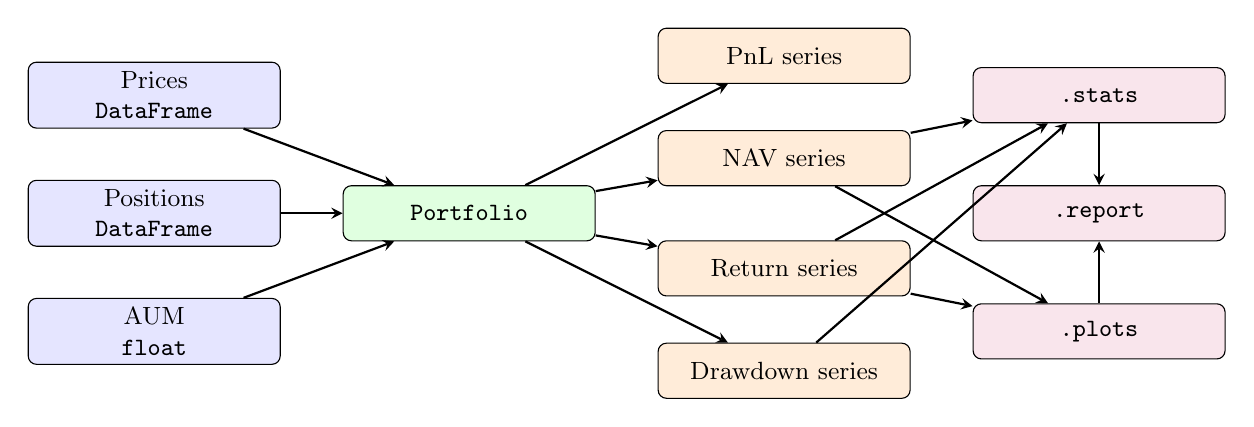
\begin{tikzpicture}[
  box/.style={draw, rounded corners=3pt, minimum width=3.2cm,
              minimum height=0.7cm, align=center, font=\small},
  arr/.style={->, thick, >=stealth}
]
% Column 1: inputs
\node[box, fill=blue!10]  (prices)   at (0,4)    {Prices \\ \texttt{DataFrame}};
\node[box, fill=blue!10]  (pos)      at (0,2.5)  {Positions \\ \texttt{DataFrame}};
\node[box, fill=blue!10]  (aum)      at (0,1)    {AUM \\ \texttt{float}};
% Column 2: Portfolio
\node[box, fill=green!12] (pf)       at (4,2.5)  {\texttt{Portfolio}};
% Column 3: derived series
\node[box, fill=orange!15](pnl)      at (8,4.5)  {PnL series};
\node[box, fill=orange!15](nav)      at (8,3.2)  {NAV series};
\node[box, fill=orange!15](ret)      at (8,1.8)  {Return series};
\node[box, fill=orange!15](dd)       at (8,0.5)  {Drawdown series};
% Column 4: facades
\node[box, fill=purple!10](stats)    at (12,4)   {\texttt{.stats}};
\node[box, fill=purple!10](report)   at (12,2.5) {\texttt{.report}};
\node[box, fill=purple!10](plots)    at (12,1)   {\texttt{.plots}};
% Arrows
\draw[arr] (prices) -- (pf);
\draw[arr] (pos)    -- (pf);
\draw[arr] (aum)    -- (pf);
\draw[arr] (pf) -- (pnl);
\draw[arr] (pf) -- (nav);
\draw[arr] (pf) -- (ret);
\draw[arr] (pf) -- (dd);
\draw[arr] (nav) -- (stats);
\draw[arr] (ret) -- (stats);
\draw[arr] (dd)  -- (stats);
\draw[arr] (nav) -- (plots);
\draw[arr] (ret) -- (plots);
\draw[arr] (stats) -- (report);
\draw[arr] (plots) -- (report);
\end{tikzpicture}
\caption{Data flow from raw inputs through \texttt{Portfolio} to the analytics facades.}
\label{fig:dataflow}
\end{figure}

\subsection{Facade Pattern}

Both \texttt{Portfolio} and \texttt{Data} expose three facade properties:
\texttt{.stats}, \texttt{.plots}, and \texttt{.report} (or \texttt{.reports}
on \texttt{Data}).  These facades are thin delegation objects constructed lazily
on first access.  This design keeps the primary classes lightweight while
providing rich secondary surfaces.

% ==========================================================================
\section{Statistical Metrics}
\label{sec:stats}
% ==========================================================================

Let $\{r_t\}_{t=1}^{T}$ denote the time series of $T$ period returns and let
$f$ denote the number of periods per year (e.g.\ $f = 252$ for daily returns,
$f = 52$ for weekly, $f = 12$ for monthly).  Unless stated otherwise, all
series are excess returns net of a risk-free rate $r_f$.

\subsection{Descriptive Statistics}

\paragraph{Average return.}
\begin{equation}
  \bar{r} = \frac{1}{T} \sum_{t=1}^{T} r_t.
\end{equation}

\paragraph{Volatility.}
Annualised realised volatility is
\begin{equation}
  \sigma = \sqrt{f} \cdot \sqrt{\frac{1}{T-1} \sum_{t=1}^{T}(r_t - \bar{r})^2}.
\end{equation}

\paragraph{Skewness and excess kurtosis.}
\begin{equation}
  \text{skew} = \frac{1}{T}\sum_{t=1}^{T}\left(\frac{r_t - \bar{r}}{\hat\sigma}\right)^3,
  \qquad
  \text{kurt} = \frac{1}{T}\sum_{t=1}^{T}\left(\frac{r_t - \bar{r}}{\hat\sigma}\right)^4 - 3,
\end{equation}
where $\hat\sigma$ is the sample standard deviation (without the $\sqrt{f}$
annualisation factor).

\paragraph{Win rate.}
\begin{equation}
  \text{WinRate} = \frac{|\{t : r_t > 0\}|}{T}.
\end{equation}

\paragraph{Payoff and profit ratios.}
Let $W = \{t : r_t > 0\}$ and $L = \{t : r_t < 0\}$.  Then
\begin{equation}
  \text{PayoffRatio} = \frac{\bar{r}_W}{|\bar{r}_L|}, \qquad
  \text{ProfitFactor} = \frac{\sum_{t \in W} r_t}{\left|\sum_{t \in L} r_t\right|},
\end{equation}
where $\bar{r}_W$ and $\bar{r}_L$ are the conditional averages over winning and
losing periods respectively.

\paragraph{Gain-to-pain ratio.}
\begin{equation}
  \text{GtP} = \frac{\sum_{t=1}^{T} r_t}{\sum_{t \in L} |r_t|}.
\end{equation}

\paragraph{Exposure.}
The fraction of periods in which the strategy holds a non-zero position:
\begin{equation}
  \text{Exposure} = \frac{|\{t : r_t \neq 0\}|}{T}.
\end{equation}

\subsection{Risk Metrics}

\paragraph{Value at Risk.}
The parametric Cornish–Fisher VaR at confidence level $\alpha$ is
\begin{equation}
  \mathrm{VaR}_\alpha = -\left(\bar{r} + z_\alpha^{\mathrm{CF}} \cdot \hat\sigma\right),
\end{equation}
where the Cornish–Fisher expansion \citep{cornish1960} adjusts the standard
normal quantile $z_\alpha$ for skewness $s$ and excess kurtosis $k$:
\begin{equation}
  z_\alpha^{\mathrm{CF}} = z_\alpha
    + \frac{z_\alpha^2 - 1}{6}\,s
    + \frac{z_\alpha^3 - 3z_\alpha}{24}\,k
    - \frac{2z_\alpha^3 - 5z_\alpha}{36}\,s^2.
\end{equation}

\paragraph{Conditional Value at Risk (Expected Shortfall).}
\begin{equation}
  \mathrm{CVaR}_\alpha = -\E[r_t \mid r_t \leq -\mathrm{VaR}_\alpha].
\end{equation}

\paragraph{Kelly criterion.}
The continuous-time Kelly fraction under a Gaussian return assumption is
\begin{equation}
  k^* = \frac{\bar{r}}{\hat\sigma^2}.
\end{equation}

\subsection{Drawdown Analysis}

Let $p_t = \prod_{s=1}^{t}(1 + r_s)$ denote the NAV indexed to~1 at inception.
The \emph{high-water mark} is
\begin{equation}
  h_t = \max_{s \leq t}\, p_s,
\end{equation}
and the drawdown at time $t$ is
\begin{equation}
  d_t = \frac{h_t - p_t}{h_t} \;\in\; [0, 1).
\end{equation}

\paragraph{Maximum drawdown.}
\begin{equation}
  \mathrm{MDD} = \max_{t \leq T}\, d_t.
\end{equation}

\paragraph{Maximum drawdown duration.}
The longest continuous interval $[t_1, t_2]$ such that $p_t < h_{t_1-1}$ for
all $t \in [t_1, t_2]$.

\paragraph{Average drawdown.}
The mean drawdown depth over all underwater periods.

\subsection{Risk-Adjusted Ratios}

\paragraph{Sharpe ratio \citep{sharpe1966}.}
\begin{equation}
  \mathrm{SR} = \frac{\bar{r}}{\hat\sigma / \sqrt{f}} = \frac{\bar{r}\,\sqrt{f}}{\hat\sigma}.
\end{equation}

\paragraph{Asymptotic Sharpe variance.}
Under mild regularity conditions \citep{bailey2012} the sample Sharpe ratio
$\sr$ has variance
\begin{equation}
  \Var(\sr) \approx \frac{1}{T}\left(1 + \frac{\mathrm{skew}\cdot\sr}{2} +
  \frac{(\mathrm{kurt}-3)\cdot\sr^2}{4}\right).
\end{equation}

\paragraph{Probabilistic Sharpe ratio.}
The probability that the true Sharpe ratio exceeds a benchmark $\mathrm{SR}^*$:
\begin{equation}
  \mathrm{PSR}(\mathrm{SR}^*) = \Phi\!\left(
    \frac{(\sr - \mathrm{SR}^*)\sqrt{T-1}}{\sqrt{1 - \mathrm{skew}\cdot\sr +
    \frac{\mathrm{kurt}-1}{4}\cdot\sr^2}}
  \right),
\end{equation}
where $\Phi$ is the standard normal CDF.

\paragraph{Sortino ratio \citep{sortino1994}.}
\begin{equation}
  \mathrm{Sortino} = \frac{\bar{r}\,\sqrt{f}}{\sigma_d}, \qquad
  \sigma_d = \sqrt{\frac{1}{T}\sum_{t=1}^{T}\min(r_t, 0)^2}.
\end{equation}

\paragraph{Calmar ratio \citep{calmar1991}.}
\begin{equation}
  \mathrm{Calmar} = \frac{\bar{r}\,f}{\mathrm{MDD}}.
\end{equation}

\paragraph{Recovery factor.}
\begin{equation}
  \mathrm{RF} = \frac{p_T - 1}{\mathrm{MDD}}.
\end{equation}

\paragraph{Risk–return ratio.}
\begin{equation}
  \mathrm{RRR} = \frac{\bar{r}}{\mathrm{CVaR}_\alpha}.
\end{equation}

\subsection{Concentration Metrics}

The Herfindahl--Hirschman Index \citep{herfindahl1950} applied to the
cross-sectional distribution of signed returns:
\begin{equation}
  \mathrm{HHI}^+ = \sum_{t \in W}\left(\frac{r_t}{\sum_{s \in W} r_s}\right)^2,
  \qquad
  \mathrm{HHI}^- = \sum_{t \in L}\left(\frac{r_t}{\sum_{s \in L} r_s}\right)^2.
\end{equation}
Values close to $1/|W|$ (or $1/|L|$) indicate uniform dispersion; values
close to~1 indicate concentration in a single period.

\subsection{Benchmark and Factor Analytics}

Let $\{b_t\}$ be a benchmark return series of the same length.  Define active
returns $a_t = r_t - b_t$.

\paragraph{Information ratio.}
\begin{equation}
  \mathrm{IR} = \frac{\bar{a}\,\sqrt{f}}{\hat\sigma_a},
  \qquad \hat\sigma_a = \sqrt{\frac{1}{T-1}\sum_t(a_t - \bar{a})^2}.
\end{equation}

\paragraph{Alpha and Beta \citep{jensen1968}.}
Estimated by OLS of $r_t = \alpha + \beta\,b_t + \varepsilon_t$:
\begin{align}
  \hat\beta &= \frac{\Cov(r_t,\,b_t)}{\Var(b_t)}, \\
  \hat\alpha &= \bar{r} - \hat\beta\,\bar{b}.
\end{align}

\paragraph{R-squared.}
\begin{equation}
  R^2 = 1 - \frac{\sum_t(r_t - \hat\alpha - \hat\beta\,b_t)^2}{\sum_t(r_t - \bar r)^2}.
\end{equation}

\paragraph{Capture ratios.}
\begin{equation}
  \mathrm{UpCapture} = \frac{\bar{r}_{b>0}}{\bar{b}_{b>0}}, \qquad
  \mathrm{DownCapture} = \frac{\bar{r}_{b<0}}{\bar{b}_{b<0}},
\end{equation}
where subscripts denote conditioning on benchmark return sign.

\subsection{Compound Return Metrics}

\paragraph{Compound return.}
\begin{equation}
  \mathrm{Comp} = \prod_{t=1}^{T}(1 + r_t) - 1.
\end{equation}

\paragraph{Geometric holding period return (GHPR).}
The per-period geometric mean return, equivalent to the $T$-th root of the
terminal wealth ratio:
\begin{equation}
  \mathrm{GHPR} = \left(\prod_{t=1}^{T}(1 + r_t)\right)^{1/T} - 1.
\end{equation}

\paragraph{Compound annual growth rate.}
\begin{equation}
  \mathrm{CAGR} = \left(\prod_{t=1}^{T}(1 + r_t)\right)^{f/T} - 1.
\end{equation}

\subsection{Omega Ratio}

The Omega ratio \citep{keating2002} measures the probability-weighted ratio of
gains to losses relative to a threshold return $\tau$:
\begin{equation}
  \Omega(\tau) = \frac{\int_\tau^\infty [1 - F(r)]\,\mathrm{d}r}
                      {\int_{-\infty}^\tau F(r)\,\mathrm{d}r},
\end{equation}
where $F$ is the empirical cumulative distribution of returns.  In the
discrete-sample implementation with $\tau = r_f$:
\begin{equation}
  \Omega = \frac{\sum_{t : r_t > \tau}(r_t - \tau)}
                {\sum_{t : r_t \leq \tau}(\tau - r_t)}.
\end{equation}

\subsection{Autocorrelation Metrics}

\paragraph{Autocorrelation at lag $\ell$.}
\begin{equation}
  \rho(\ell) = \frac{\sum_{t=\ell+1}^{T}(r_t - \bar{r})(r_{t-\ell} - \bar{r})}
                    {\sum_{t=1}^{T}(r_t - \bar{r})^2}.
\end{equation}

\paragraph{Autocorrelation penalty (Lo, 2002).}
Under serially correlated returns, the Sharpe ratio estimator has inflated
variance.  The autocorrelation penalty scales the Sharpe ratio to correct for
this bias:
\begin{equation}
  \text{penalty} = \sqrt{1 + 2\sum_{\ell=1}^{\min(T-1,\,\lfloor T/5\rfloor)}
    \rho(\ell)\,\frac{T - \ell}{T}}.
\end{equation}
\texttt{smart\_sharpe()} and \texttt{smart\_sortino()} divide the standard
Sharpe and Sortino estimates by this factor.

\subsection{Rolling Analytics}

jQuantStats computes rolling variants of the Sharpe ratio, Sortino ratio,
volatility, and benchmark greeks (alpha and beta) over a configurable
look-back window $w$:
\begin{equation}
  \mathrm{SR}_t^{(w)} = \frac{\bar{r}_{t-w+1:t}\,\sqrt{f}}
                              {\hat\sigma_{t-w+1:t}}.
\end{equation}
Rolling computations are implemented via Polars' native
\texttt{rolling\_mean} and \texttt{rolling\_std} operations, which execute in
compiled Rust and avoid Python-level loops.

% ==========================================================================
\section{Tilt/Timing Attribution}
\label{sec:attribution}
% ==========================================================================

The Brinson--Hood--Beebower \citep{brinson1986} framework decomposes active
return into components attributable to asset allocation and security selection.
jQuantStats adapts this to a time-series context and refers to the two
components as \emph{tilt} and \emph{timing}.

\paragraph{Setup.}
Let $w_{i,t}$ denote the weight of instrument~$i$ on day~$t$ as a fraction of
AUM, $w_{i,t}^b$ the benchmark weight, and $r_{i,t}$ the return of instrument~$i$.
Portfolio return and benchmark return are
\begin{equation}
  r_t^p = \sum_i w_{i,t}\,r_{i,t}, \qquad r_t^b = \sum_i w_{i,t}^b\,r_{i,t}.
\end{equation}

\paragraph{Tilt.}
The tilt component captures the contribution from holding average overweights
or underweights relative to the benchmark:
\begin{equation}
  \text{Tilt}_t = \sum_i \bigl(\bar{w}_i - \bar{w}_i^b\bigr)\,r_{i,t},
\end{equation}
where $\bar{w}_i = T^{-1}\sum_t w_{i,t}$ is the time-averaged weight.

\paragraph{Timing.}
The timing component captures the contribution from dynamic weight deviations
around the time-average:
\begin{equation}
  \text{Timing}_t = \sum_i \bigl(w_{i,t} - \bar{w}_i\bigr)\,r_{i,t}.
\end{equation}

\begin{remark}
By construction, $r_t^p - r_t^b = \text{Tilt}_t + \text{Timing}_t + \varepsilon_t$,
where $\varepsilon_t$ is a residual driven by the benchmark's own active
weight deviations.  For equal-weight benchmarks with $w_{i,t}^b \equiv 1/N$
this residual vanishes.
\end{remark}

The library exposes this decomposition through \texttt{Portfolio.tilt},
\texttt{Portfolio.timing}, and \texttt{Portfolio.tilt\_timing\_decomp()}.

% ==========================================================================
\section{Transaction Cost Models}
\label{sec:costs}
% ==========================================================================

jQuantStats implements two independent, additive transaction cost models
encapsulated in \texttt{CostModel}.

\subsection{Model~A: Per-Unit Cost}

Each time a position changes by $\Delta n_{i,t}$ units, a cost of
$c_{\text{unit}}$ per unit is incurred:
\begin{equation}
  C_t^A = c_{\text{unit}} \sum_i |\Delta n_{i,t}|.
\end{equation}
This model is appropriate for instruments with fixed brokerage commissions,
stamp duty, or exchange fees quoted per share.  It is constructed with
\texttt{CostModel.per\_unit(c)}.

\subsection{Model~B: Turnover Basis Points}

Each unit of one-way portfolio turnover incurs a cost of $c_{\text{bps}}$
basis points of AUM:
\begin{equation}
  C_t^B = \frac{c_{\text{bps}}}{10\,000} \cdot \mathrm{AUM}_t \cdot
          \frac{\sum_i |\Delta w_{i,t}|}{2},
\end{equation}
where $\Delta w_{i,t}$ is the change in weight of instrument~$i$.  This model
is appropriate for strategies that are sized in terms of portfolio weight and
where the dominant cost is the bid–offer spread.  It is constructed with
\texttt{CostModel.turnover\_bps(c)}.

\begin{remark}
The two models are mutually exclusive at construction time: a \texttt{CostModel}
may have a non-zero per-unit cost or a non-zero turnover-bps cost, but not both.
This constraint avoids accidental double-counting.
\end{remark}

\subsection{Cost-Adjusted Returns}

\texttt{Portfolio.cost\_adjusted\_returns()} subtracts $C_t / \mathrm{AUM}_t$
from the gross return series to produce a net-of-cost return stream on which
all downstream metrics are computed.  The method
\texttt{Portfolio.trading\_cost\_impact\_plot(max\_bps)} sweeps the
turnover-bps parameter from~0 to \texttt{max\_bps} and plots how key metrics
(Sharpe ratio, Calmar ratio, annualised return) degrade with increasing cost,
providing practitioners with a breakeven cost analysis.

% ==========================================================================
\section{Visualisation and Reporting}
\label{sec:plots}
% ==========================================================================

\subsection{Data Plots}

\texttt{DataPlots.plot\_snapshot()} renders a three-panel dashboard:
\begin{enumerate}
  \item Cumulative return (linear or log scale, switchable interactively).
  \item Underwater drawdown chart.
  \item Monthly returns heatmap with calendar layout.
\end{enumerate}

\subsection{Portfolio Plots}

\texttt{PortfolioPlots} exposes the following charts.

\begin{center}
\begin{tabular}{@{}ll@{}}
\toprule
Method & Description \\
\midrule
\texttt{snapshot(log\_scale)} & NAV overlay with drawdown subplot \\
\texttt{rolling\_sharpe\_plot(window)} & Time series of $\mathrm{SR}_t^{(w)}$ \\
\texttt{rolling\_volatility\_plot(window)} & Time series of $\sigma_t^{(w)}$ \\
\texttt{annual\_sharpe\_plot()} & Per-year Sharpe ratio bar chart \\
\texttt{monthly\_returns\_heatmap()} & Calendar-style return heat map \\
\texttt{correlation\_heatmap()} & Cross-instrument correlation matrix \\
\texttt{lead\_lag\_ir\_plot(start, end)} & IR as a function of signal lag $\ell$ \\
\texttt{lagged\_performance\_plot(lags)} & Cumulative NAV for each lag $\ell$ \\
\texttt{smoothed\_holdings\_performance\_plot()} & Smoothed position PnL \\
\texttt{trading\_cost\_impact\_plot(max\_bps)} & Metric decay vs.\ cost sweep \\
\bottomrule
\end{tabular}
\end{center}

\paragraph{Lead-lag analysis.}
Given a position matrix $w_{i,t}$ derived from a signal, the lead-lag IR plot
re-evaluates portfolio performance under a lag of $\ell \in \{0,1,\ldots,L\}$
days, replacing $w_{i,t}$ with $w_{i,t-\ell}$.  A sharp degradation at small
lags confirms that the strategy's edge is genuinely predictive rather than
capacity-constrained by execution timing.

\subsection{HTML Reports}

Both \texttt{Portfolio} and \texttt{Data} expose a \texttt{.report} (or
\texttt{.reports}) facade.  Calling \texttt{.to\_html(title)} produces a
self-contained HTML file—embedding all Plotly charts inline as JavaScript—that
can be shared without external dependencies.

% ==========================================================================
\section{Annualisation and Frequency Detection}
\label{sec:annualisation}
% ==========================================================================

All ratio metrics require a value for $f$, the number of periods per year.
jQuantStats infers $f$ automatically from the median observed gap between
consecutive timestamps in the return series according to the following table.

\begin{center}
\begin{tabular}{@{}lc@{}}
\toprule
Detected frequency & $f$ \\
\midrule
Daily         & 252 \\
Weekly        & 52  \\
Bi-weekly     & 26  \\
Monthly       & 12  \\
Quarterly     & 4   \\
Annual        & 1   \\
\bottomrule
\end{tabular}
\end{center}

The caller may override $f$ by passing \texttt{periods=} to any method that
accepts it.  When computing rolling statistics, the same $f$ is used for
annualisation inside each window.

\begin{remark}
Using 252 trading days rather than 365 calendar days is standard practice in
equity portfolio analytics.  Practitioners working with futures or FX returns
that accrue daily over weekends may wish to override to~365.
\end{remark}

% ==========================================================================
\section{End-to-End Usage Example}
\label{sec:usage}
% ==========================================================================

The following listing demonstrates a representative workflow: loading data,
constructing a \texttt{Portfolio}, inspecting key metrics, running attribution,
and saving an HTML report.

\begin{lstlisting}[caption={Complete usage example.}]
import polars as pl
from jquantstats import Portfolio, CostModel

# ------------------------------------------------------------------ #
# 1. Load price and position data (example: two instruments)         #
# ------------------------------------------------------------------ #
prices = pl.read_csv("prices.csv", try_parse_dates=True)
# prices has columns: ["Date", "AAPL", "MSFT"]

positions = pl.read_csv("positions.csv", try_parse_dates=True)
# positions has columns: ["Date", "AAPL", "MSFT"]
# values are signed cash notionals in GBP

# ------------------------------------------------------------------ #
# 2. Construct the Portfolio with a 5 bps/side cost model            #
# ------------------------------------------------------------------ #
pf = Portfolio.from_cash_position(
    prices=prices,
    cash_position=positions,
    aum=10_000_000,
    cost_bps=5.0,          # 5 bps of AUM per unit of one-way turnover
)

# ------------------------------------------------------------------ #
# 3. Inspect summary statistics                                       #
# ------------------------------------------------------------------ #
print(pf.stats.summary())

# ------------------------------------------------------------------ #
# 4. Risk-adjusted ratios                                             #
# ------------------------------------------------------------------ #
print("Sharpe     :", round(pf.stats.sharpe(), 3))
print("Sortino    :", round(pf.stats.sortino(), 3))
print("Calmar     :", round(pf.stats.calmar(), 3))
print("Max DD     :", round(pf.stats.max_drawdown(), 4))
print("CVaR 5%    :", round(pf.stats.conditional_value_at_risk(), 4))
print("Kelly      :", round(pf.stats.kelly_criterion(), 4))

# ------------------------------------------------------------------ #
# 5. Benchmark attribution (if a benchmark is available)             #
# ------------------------------------------------------------------ #
bench = pl.read_csv("sp500.csv", try_parse_dates=True)["Return"]
d = pf.data  # bridge to Data API
d_with_bench = d.__class__.from_returns(d.returns, benchmark=bench)
print("Alpha      :", round(d_with_bench.stats.greeks()["alpha"], 4))
print("Beta       :", round(d_with_bench.stats.greeks()["beta"], 4))
print("IR         :", round(d_with_bench.stats.information_ratio(), 3))

# ------------------------------------------------------------------ #
# 6. Tilt / Timing decomposition                                      #
# ------------------------------------------------------------------ #
tilt, timing = pf.tilt, pf.timing
print("Tilt Sharpe  :", round(tilt.stats.sharpe(), 3))
print("Timing Sharpe:", round(timing.stats.sharpe(), 3))

# ------------------------------------------------------------------ #
# 7. Turnover summary                                                 #
# ------------------------------------------------------------------ #
print(pf.turnover_summary())

# ------------------------------------------------------------------ #
# 8. Interactive plots                                                #
# ------------------------------------------------------------------ #
pf.plots.snapshot().show()
pf.plots.rolling_sharpe_plot(window=63).show()
pf.plots.trading_cost_impact_plot(max_bps=20).show()

# ------------------------------------------------------------------ #
# 9. Save self-contained HTML report                                  #
# ------------------------------------------------------------------ #
pf.report.save("strategy_report.html", title="My Strategy")
\end{lstlisting}

% ==========================================================================
\section{Design Decisions and Limitations}
\label{sec:design}
% ==========================================================================

\subsection{Zero Pandas Dependency}

The decision to eliminate pandas from the runtime dependency graph was
deliberate.  Pandas' object-dtype columns, copy-on-write semantics, and
implicit type coercions have historically been a source of silent correctness
bugs in financial libraries.  Polars enforces strict column types, returns
immutable DataFrames by default, and provides a significantly faster execution
engine for the columnar operations that dominate portfolio analytics.

\subsection{Narwhals Boundary Layer}

Although the core is Polars-native, some users maintain existing pipelines in
pandas.  The Narwhals boundary layer allows both pandas \texttt{DataFrame}s
and Polars \texttt{DataFrame}s to be passed to factory methods.  Internally,
the library immediately converts to Polars for all computations; the
abstraction adds negligible overhead.

\subsection{Limitations}

\begin{itemize}
  \item \textbf{Single-currency.}  The library does not model multi-currency
    portfolios or FX hedging.  All cash flows are assumed to be denominated
    in a single base currency.
  \item \textbf{Linear cost models only.}  Market impact models (e.g.\
    Almgren–Chriss) and non-linear fee schedules are not yet implemented.
  \item \textbf{No live data integration.}  jQuantStats is a purely offline
    analytics library.  Real-time data feeds must be managed by the caller.
  \item \textbf{Parametric VaR.}  The Cornish–Fisher expansion is an
    approximation that may understate tail risk for highly non-Gaussian
    return distributions.  Historical or Monte Carlo simulation-based VaR
    is not implemented.
\end{itemize}

% ==========================================================================
\section{Conclusion}
\label{sec:conclusion}
% ==========================================================================

jQuantStats provides a modern, type-safe, and performant foundation for
portfolio analytics in Python.  By adopting Polars as the compute backend,
Plotly as the visualisation layer, and a clean two-class public API, it
addresses the limitations of the previous generation of pandas-based tools
while retaining full compatibility via the Narwhals boundary layer.

The mathematical definitions in Section~\ref{sec:stats} give practitioners
an unambiguous reference for the precise computation of each metric.  The
Brinson-style tilt/timing decomposition in Section~\ref{sec:attribution} and
the two-factor cost model in Section~\ref{sec:costs} extend the library beyond
simple performance measurement into attribution and cost analysis.

Future development priorities include multi-currency support, non-linear cost
modelling, and expanded factor attribution capabilities.

% ==========================================================================
% Bibliography
% ==========================================================================
\bibliographystyle{plainnat}
\bibliography{jquantstats}

% ==========================================================================
% Appendices
% ==========================================================================
\appendix

\section{API Quick Reference}
\label{app:api}

\subsection{Portfolio — Key Properties and Methods}

\begin{longtable}{@{}p{5.5cm}p{8.5cm}@{}}
\toprule
Property / Method & Description \\
\midrule
\endhead
\texttt{.profits} & Per-instrument daily PnL DataFrame \\
\texttt{.profit} & Aggregate daily PnL series \\
\texttt{.nav\_accumulated} & Linearly accumulated NAV series \\
\texttt{.nav\_compounded} & Compounded NAV series \\
\texttt{.returns} & Daily return series \\
\texttt{.monthly} & Monthly return series \\
\texttt{.drawdown} & Drawdown series \\
\texttt{.highwater} & High-water mark series \\
\texttt{.tilt} & Tilt return stream (Data object) \\
\texttt{.timing} & Timing return stream (Data object) \\
\texttt{.tilt\_timing\_decomp()} & Full Brinson decomposition table \\
\texttt{.turnover} & Daily one-way turnover series \\
\texttt{.turnover\_weekly} & Weekly aggregate turnover \\
\texttt{.turnover\_summary()} & Summary statistics of turnover \\
\texttt{.cost\_adjusted\_returns()} & Net-of-cost return series \\
\texttt{.trading\_cost\_impact(max\_bps)} & Metric table across cost sweep \\
\texttt{.correlation()} & Cross-instrument return correlation matrix \\
\texttt{.stats} & Stats facade (see below) \\
\texttt{.plots} & Plots facade (see Section~\ref{sec:plots}) \\
\texttt{.report} & Report facade \\
\bottomrule
\end{longtable}

\subsection{Stats Facade — Key Methods}

\begin{longtable}{@{}p{5.5cm}p{8.5cm}@{}}
\toprule
Method & Returns \\
\midrule
\endhead
\texttt{.summary()} & Comprehensive statistics DataFrame \\
\midrule
\multicolumn{2}{@{}l@{}}{\textit{Return metrics}} \\
\texttt{.avg\_return()} & Mean period return \\
\texttt{.avg\_win()} & Mean positive-period return \\
\texttt{.avg\_loss()} & Mean negative-period return \\
\texttt{.best()} & Best single-period return \\
\texttt{.worst()} & Worst single-period return \\
\texttt{.comp()} & Compound cumulative return \\
\texttt{.geometric\_mean()} & Geometric mean period return \\
\texttt{.cagr()} & Compound annual growth rate \\
\texttt{.ghpr()} & Geometric holding period return \\
\texttt{.expected\_return(aggregate)} & Expected return (optionally aggregated) \\
\texttt{.win\_rate()} & Fraction of positive-return periods \\
\texttt{.payoff\_ratio()} & Avg win / avg loss \\
\texttt{.profit\_factor()} & Gross profit / gross loss \\
\texttt{.gain\_to\_pain\_ratio()} & Cumulative return / sum of losses \\
\texttt{.exposure()} & Fraction of non-zero return periods \\
\midrule
\multicolumn{2}{@{}l@{}}{\textit{Risk and volatility}} \\
\texttt{.volatility(series, periods, annualize)} & Realised annualised volatility \\
\texttt{.value\_at\_risk(series, sigma, alpha)} & Cornish--Fisher VaR \\
\texttt{.conditional\_value\_at\_risk()} & Expected Shortfall \\
\texttt{.kelly\_criterion()} & Optimal Kelly fraction \\
\texttt{.tail\_ratio(cutoff)} & Ratio of upper to lower tail \\
\texttt{.skew()} & Return distribution skewness \\
\texttt{.kurtosis()} & Return distribution excess kurtosis \\
\texttt{.outliers(quantile)} & Return outlier periods \\
\texttt{.remove\_outliers(quantile)} & Return series with outliers removed \\
\texttt{.outlier\_win\_ratio(quantile)} & Fraction of returns above upper quantile \\
\texttt{.outlier\_loss\_ratio(quantile)} & Fraction of returns below lower quantile \\
\midrule
\multicolumn{2}{@{}l@{}}{\textit{Drawdown}} \\
\texttt{.max\_drawdown(series)} & Maximum drawdown \\
\texttt{.max\_drawdown\_duration()} & Duration of worst drawdown \\
\texttt{.avg\_drawdown(series)} & Mean drawdown over underwater periods \\
\texttt{.drawdown\_details()} & Per-drawdown-period table per asset \\
\texttt{.calmar(series, periods)} & Calmar ratio \\
\texttt{.recovery\_factor(series)} & Total return / max drawdown \\
\midrule
\multicolumn{2}{@{}l@{}}{\textit{Risk-adjusted ratios}} \\
\texttt{.sharpe(series, periods)} & Annualised Sharpe ratio \\
\texttt{.sharpe\_variance()} & Asymptotic variance of Sharpe estimate \\
\texttt{.probabilistic\_sharpe\_ratio(sr*)} & Probabilistic Sharpe ratio \\
\texttt{.probabilistic\_sortino\_ratio()} & Probabilistic Sortino ratio \\
\texttt{.probabilistic\_adjusted\_sortino\_ratio()} & Probabilistic adjusted Sortino ratio \\
\texttt{.probabilistic\_ratio(base)} & Generalised probabilistic ratio \\
\texttt{.sortino(series, periods)} & Annualised Sortino ratio \\
\texttt{.adjusted\_sortino()} & Sortino / $\sqrt{2}$ \\
\texttt{.smart\_sharpe()} & Sharpe with autocorrelation penalty \\
\texttt{.smart\_sortino()} & Sortino with autocorrelation penalty \\
\texttt{.omega()} & Omega ratio \\
\texttt{.treynor\_ratio()} & Treynor ratio \\
\texttt{.ulcer\_index()} & Ulcer Index \\
\texttt{.serenity\_index()} & Serenity Index \\
\texttt{.common\_sense\_ratio()} & Common Sense Ratio \\
\texttt{.cpc\_index()} & CPC Index \\
\midrule
\multicolumn{2}{@{}l@{}}{\textit{Benchmark and factor analytics}} \\
\texttt{.information\_ratio()} & Information ratio vs benchmark \\
\texttt{.greeks()} & Dict with alpha and beta \\
\texttt{.r\_squared(series, bench)} & $R^2$ of return regression \\
\texttt{.up\_capture()} & Return capture during up-market periods \\
\texttt{.down\_capture()} & Return capture during down-market periods \\
\midrule
\multicolumn{2}{@{}l@{}}{\textit{Autocorrelation and serial dependence}} \\
\texttt{.autocorr(lag)} & Pearson autocorrelation at lag $\ell$ \\
\texttt{.acf(nlags)} & Full autocorrelation function as DataFrame \\
\texttt{.autocorr\_penalty()} & Autocorrelation penalty factor \\
\midrule
\multicolumn{2}{@{}l@{}}{\textit{Concentration}} \\
\texttt{.hhi\_positive()} & HHI concentration of gains \\
\texttt{.hhi\_negative()} & HHI concentration of losses \\
\midrule
\multicolumn{2}{@{}l@{}}{\textit{Rolling analytics}} \\
\texttt{.rolling\_sharpe(window)} & Rolling Sharpe ratio series \\
\texttt{.rolling\_sortino(window)} & Rolling Sortino ratio series \\
\texttt{.rolling\_volatility(window)} & Rolling volatility series \\
\texttt{.rolling\_greeks(window)} & Rolling alpha/beta vs benchmark \\
\midrule
\multicolumn{2}{@{}l@{}}{\textit{Period breakdown}} \\
\texttt{.monthly\_returns(eoy, compounded)} & Per-month return table \\
\texttt{.monthly\_win\_rate()} & Win rate aggregated by month \\
\texttt{.annual\_breakdown()} & Per-year statistics table \\
\texttt{.distribution(compounded)} & Return distribution by period type \\
\texttt{.compare(aggregate)} & Strategy vs benchmark return table \\
\bottomrule
\end{longtable}

\subsection{CostModel — Factory Methods}

\begin{center}
\begin{tabular}{@{}p{5.5cm}p{8.5cm}@{}}
\toprule
Factory & Description \\
\midrule
\texttt{CostModel.per\_unit(c)} & £$c$ per share traded (Model A) \\
\texttt{CostModel.turnover\_bps(c)} & $c$ bps of AUM per unit of one-way turnover (Model B) \\
\bottomrule
\end{tabular}
\end{center}

\end{document}
